%%
%% Copyright 2019-2024 Elsevier Ltd
%%
%% This file is part of the 'CAS Bundle'.
%% --------------------------------------
%%
%% It may be distributed under the conditions of the LaTeX Project Public
%% License, either version 1.3c of this license or (at your option) any
%% later version.  The latest version of this license is in
%%    http://www.latex-project.org/lppl.txt
%% and version 1.3c or later is part of all distributions of LaTeX
%% version 1999/12/01 or later.
%%
%% The list of all files belonging to the 'CAS Bundle' is
%% given in the file `manifest.txt'.
%%
%% Template article for cas-sc documentclass for
%% double column output.

\documentclass[a4paper,fleqn]{cas-sc}

% If the frontmatter runs over more than one page
% use the longmktitle option.

%\documentclass[a4paper,fleqn,longmktitle]{cas-sc}

\usepackage[authoryear,longnamesfirst]{natbib}
\usepackage{booktabs}
\usepackage{amsmath,amssymb}
\usepackage{graphicx}
\usepackage{pgfplots}
\pgfplotsset{compat=1.18}
\newcommand{\std}[1]{$\,\pm\,$#1}

\begin{document}
\let\WriteBookmarks\relax
\def\floatpagepagefraction{1}
\def\textpagefraction{.001}
\shorttitle{On Image Classification with Random Convolutional Kernels}
\shortauthors{Lock and Bonenberger}

% Main title of the paper
\title[mode=title]{2D Image Classification with Random Convolutional Kernels: A ROCKET-Based Approach}

% First author
\author[1]{Felicitas Lock}
\cormark[1]
\credit{Conceptualization, Methodology, Software, Investigation, Writing -- original draft}

\affiliation[1]{organization={Faculty of Electrical Engineering and Computer Science, Ravensburg-Weingarten University of Applied Sciences},
                city={Weingarten},
                country={Germany}}

% Second author
\author[1]{Christopher Bonenberger}
\credit{Supervision, Writing -- review \& editing}

% Corresponding author text
\cortext[1]{Corresponding author}

% Here goes the abstract
\begin{abstract}
Deep learning achieves strong performance in image classification but often requires costly training and substantial computational resources. This paper explores a lightweight alternative by adapting the ROCKET framework from time-series classification to two-dimensional image data. The proposed 2D-ROCKET approach applies large banks of random 2D convolutional kernels and summarizes their responses using simple aggregation statistics, enabling efficient feature extraction without learned filters and, structurally, without the stacked, hierarchical multi-scale composition that gives deep CNNs their representational power. MNIST and CIFAR-10 are used here not as target applications but as controlled, well-understood benchmarks to probe the method's ceiling: preserving spatial structure with 2D kernels improves performance compared to flattened 1D variants, and a final configuration (5,000 mixed-scale kernels, moderate dilation, valid padding) reaches 99.41\% accuracy on MNIST and 73.43\% on CIFAR-10, slightly ahead of a deliberately shallow, two-layer CNN baseline on both benchmarks and far ahead of a linear SVM, at a fraction of the SVM's training time. This should not be read as evidence that 2D-ROCKET rivals deep CNNs in general: the shallow baseline itself has little of the multi-scale hierarchical depth that distinguishes modern, deeper architectures, which were out of scope for this comparison. Object recognition on natural images is, in any case, not the domain 2D-ROCKET is proposed for: a proof-of-concept on the texture-dominated KTH-TIPS dataset (94.7\% accuracy, versus 43.5\%/52.4\% for SVM/CNN) indicates that the method's real niche is texture-like, repetitive-pattern imagery -- material and surface textures, inspection data, or structured surface signals -- where classification does not depend on the multi-scale, compositional object structure that only deep, hierarchical architectures can capture. This texture-domain scoping is then tested directly, not just asserted, on three independently sourced, real-world datasets -- industrial surface-defect inspection (NEU), a texture-attribute benchmark (DTD), and chest X-ray pneumonia screening -- each evaluated over ten random seeds with paired significance testing rather than the single runs used above. 2D-ROCKET wins significantly on the two texture-dominated datasets (NEU, DTD) and loses significantly, by a smaller margin, only on the non-texture, localized-pathology chest X-ray task; the reason -- that global feature pooling discards the positional information a diagnosis in that task depends on -- is tested rather than merely proposed, by adding a previously unimplemented positional-pooling feature (LSPV) that closes the chest X-ray gap to statistical indistinguishability at negligible extra cost, with a capacity-matched control attributing roughly three-quarters of that gain specifically to the restored positional resolution rather than to the added feature capacity alone. A further test on genuine 1D time series -- a freshly implemented, Dempster-et-al.-faithful 1D-ROCKET applied to raw Sentinel-1 SAR echo lines for radio-frequency-interference detection, a real, deliberately small-sample (216-example) problem -- replicates 1D-ROCKET's advantage over a linear SVM but not over a CNN, consistent with the same texture-vs-localized-anomaly distinction rather than sample size alone driving where ROCKET-family methods have an edge. Overall, 2D-ROCKET provides a simple, training-efficient, and interpretable baseline, and highlights random convolutional feature extraction as a promising direction for lightweight, texture-oriented image classification, rather than as a competitor to deep CNNs on general object recognition.
\end{abstract}

% Research highlights
\begin{highlights}
\item Adapts ROCKET's random-kernel, statistics-based paradigm from 1D time series to 2D images.
\item Systematic ablations isolate the effect of feature statistics, 1D vs.\ 2D kernels, padding, preprocessing, and kernel budget.
\item Final 2D-ROCKET reaches 99.41\% (MNIST) / 73.43\% (CIFAR-10) without any gradient-based training.
\item Trains in seconds to minutes, versus hours for a linear SVM baseline, while beating it decisively in accuracy.
\item Slightly beats a deliberately shallow CNN baseline, but as a flat, single-stage method it has no mechanism for the multi-scale composition of deeper CNNs; proposed instead for texture-dominated imagery, where a KTH-TIPS proof-of-concept reaches 94.7\%.
\item A ten-seed, paired-significance real-world evaluation (NEU, DTD, Chest X-Ray) confirms the texture-domain scoping rather than assuming it: 2D-ROCKET wins significantly on texture-dominated NEU/DTD and loses significantly, more narrowly, on non-texture Chest X-Ray.
\item Adding a previously unimplemented positional-pooling feature (LSPV) closes the Chest X-Ray gap to non-significance ($p=0.22$) at no meaningful runtime cost, directly confirming the mechanistic explanation for that one loss.
\item A genuine 1D-ROCKET, freshly implemented and applied to real Sentinel-1 raw radar time series for radio-frequency-interference detection, beats a linear SVM but not a CNN on this small-sample (216-example) task -- extending the texture-vs-localized-anomaly account to a non-image domain and showing that low data alone does not predict a ROCKET advantage.
\end{highlights}

% Keywords
\begin{keywords}
ROCKET \sep random convolutional kernels \sep image classification \sep lightweight machine learning \sep feature extraction \sep texture classification
\end{keywords}

\maketitle

\section{Introduction}\label{sec:intro}

Image classification has become a central task in machine learning, with deep learning models achieving remarkable accuracy across a wide range of datasets. Classic machine learning algorithms, both on images and on time series, often require expensive feature-engineering steps, resulting in a demand for high computing effort and correspondingly powerful hardware \citep{ismailfawaz2019deep}. Moreover, these models often come with large memory requirements and limited interpretability. Exploring alternative approaches that are computationally efficient, lightweight, and conceptually simple is therefore of growing interest.

RandOm Convolutional KErnel Transform (ROCKET) is a method originally developed for time-series classification that offers high efficiency through large banks of random convolutional kernels combined with simple aggregation features and a linear classifier \citep{dempster2020rocket}. Investigating whether this idea can be transferred to image data may yield insights into efficient, non-deep alternatives for image classification.

The main objective of this work is to investigate whether ROCKET-style feature extraction can be effectively adapted to image classification. Concretely, we (i) design a ROCKET-inspired 2D feature-extraction pipeline for images using random convolutional kernels and simple aggregation statistics, (ii) analyze the impact of kernel size, dilation, kernel count, padding, and feature selection through controlled ablations, (iii) evaluate the resulting pipeline, termed 2D-ROCKET, on MNIST and CIFAR-10, (iv) compare it against a minimal 1D-ROCKET baseline, a linear SVM, and a lightweight CNN, and (v) test the texture-domain scope this comparison points toward against a lightweight CNN on three independent, real-world datasets under a properly powered, multi-seed statistical protocol, rather than resting that scoping claim on single-run comparisons alone.

The scope is deliberately restricted: all convolutional kernels remain fixed after random initialization, hyperparameter search is limited to small predefined grids, and comparisons are made against lightweight rather than state-of-the-art baselines. The goal is not to outperform modern deep networks, but to isolate the effect of spatially structured random convolutions and quantify the resulting accuracy/cost trade-offs.

A related but separate scoping point concerns the target application. MNIST and CIFAR-10 are used here because they are standard, well-characterized benchmarks that make the ablations reproducible and comparable to prior work -- not because natural-object recognition is where 2D-ROCKET is expected to be competitive. A deep CNN builds its representation through several stacked convolutional and pooling layers, composing local edges into increasingly abstract, multi-scale object parts; 2D-ROCKET, by construction, performs a single flat feature-extraction stage with no learned composition across layers (Sec.~\ref{sec:related}). The CNN baseline used for comparison in this paper is deliberately shallow (two convolutional layers, Sec.~\ref{sec:methods}) to keep model complexity comparable across baselines, and consequently makes only limited use of the deep, multi-scale hierarchy that distinguishes modern CNN architectures such as ResNets -- which, along with other deep or state-of-the-art models, are explicitly out of scope here. 2D-ROCKET should therefore not be expected to approach the accuracy of genuinely deep, multi-scale networks on datasets like CIFAR-10, where distinguishing object classes benefits from exactly this kind of hierarchical structure, even where it matches or slightly exceeds the shallow baseline tested here (Sec.~\ref{sec:results}). The method is instead proposed for texture-dominated or otherwise spatially repetitive image data -- surface, material, or inspection imagery -- where classification relies on local, statistically distinctive patterns rather than on composed object hierarchies, and where a flat random-feature bank can plausibly substitute for learned depth. CIFAR-10 is included primarily as a stress test against object-recognition structure that 2D-ROCKET cannot represent, while the texture-oriented case is examined directly in Sec.~\ref{sec:results} via a proof-of-concept on KTH-TIPS and, at greater length and with a ten-seed statistical protocol, via three independent real-world datasets in Sec.~\ref{sec:realworld}.

This paper addresses three research questions: (i) how well does a ROCKET-style 2D feature-extraction approach perform on image classification compared to simple baselines, (ii) how do key design choices -- kernel size, dilation, kernel count, and selected aggregation features -- influence performance and computational cost, and (iii) what are the practical advantages, limitations, and application scenarios of the resulting 2D-ROCKET approach.

\section{Related Work}\label{sec:related}

\textbf{Classical and lightweight approaches.} Before the deep learning era, image classification commonly combined handcrafted feature descriptors with classical classifiers. Histogram of Oriented Gradients (HOG) summarizes gradient magnitude and direction in local cells \citep{dalal2005histograms}, while Local Binary Patterns (LBP) encode local texture via thresholded neighborhoods \citep{pietikainen2011local}. Both are typically paired with a Support Vector Machine (SVM) \citep{cortes1995support}, forming a well-understood, interpretable baseline. Lightweight convolutional networks, including shallow CNNs (SCNNs), bridge the gap between full deep networks and classical pipelines by using few convolutional layers and simple pooling while retaining learned, task-specific filters \citep{lei2019shallow}. CNNs remain the dominant approach for state-of-the-art image classification \citep{krichen2023cnn}, but their computational and memory cost motivates the search for lighter alternatives.

\textbf{ROCKET and its variants.} ROCKET extracts features from time series using a large ensemble (typically $\geq$10{,}000) of randomly initialized, fixed convolutional kernels, summarized via the Proportion of Positive Values (PPV) and the maximum activation (Max), and classified with a linear Ridge classifier \citep{dempster2020rocket}. The reliance on a large number of independent random kernels can be linked to the Johnson--Lindenstrauss lemma, which suggests that sufficiently many random projections approximately preserve pairwise distances \citep{ghojogh2021johnson}. Follow-up work improved computational efficiency and determinism: MiniROCKET restricts kernel weights to two values and uses PPV only \citep{dempster2020minirocket}; MultiROCKET adds first-order differences and three further pooling statistics -- Mean Positive Value (MPV), Mean Index of Positive Values (MIPV), and Local Share of Positive Values (LSPV) \citep{tan2022multirocket}; Hydra introduces a dictionary-style kernel-competition mechanism \citep{dempster2022hydra}. This work adopts the MultiROCKET-style statistics (MPV, MIPV, LSPV) as candidate features for the 2D setting, since they are inexpensive and plausibly informative for spatially structured data.

\textbf{Random convolutions on images.} The idea of random projections and random convolutional features for images predates ROCKET: Rahimi and Recht map inputs into a randomized low-dimensional feature space that approximates a kernel, enabling fast linear learning on non-linear problems \citep{rahimi2007random}. Random depthwise convolutional architectures combined with global pooling and a linear classifier have achieved competitive accuracy on CIFAR-10 and STL-10 \citep{xue2018random}, and random filters followed by pooling and a linear SVM have reached roughly 84\% accuracy on facial-expression classification without any filter learning \citep{ren2016facial}. Unlike these approaches, most of which retain a multi-layer, CNN-like architecture with stacked random convolutions, ROCKET performs a single, flat feature-extraction stage with simple statistical aggregation and no non-linear activations. To our knowledge, this flat ROCKET-style design has not been systematically adapted and ablated for 2D image data, which is the gap this work addresses.

\section{Methods}\label{sec:methods}

\subsection{1D-ROCKET baseline}
As a reference and sanity check, a minimal, independent 1D-ROCKET implementation follows Dempster et al.\ closely \citep{dempster2020rocket}: images are flattened row-wise, kernels of length $l$ are convolved with the flattened sequence $x$ as
\begin{equation}
(x * k)[t] = \sum_{i=0}^{l-1} x[t+i]\cdot k[i],
\end{equation}
and each kernel yields two features,
\begin{equation}
f_{\text{max}} = \max_t (x*k)[t], \qquad
f_{\text{PPV}} = \frac{1}{L-l+1}\sum_t \mathbb{1}\big((x*k)[t] > 0\big).
\end{equation}
Kernel sizes $k \in \{7,9,11\}$ and a per-kernel-group random choice between \emph{same} and \emph{valid} padding (deterministic given the seed) are used, followed by a Ridge classifier.

\subsection{2D-ROCKET design}
2D-ROCKET replaces the flattening step with genuine 2D convolutions, preserving spatial (and, for RGB inputs, channel) structure. Kernel weights are sampled with variance $2/\text{fan-in}$ (He-style initialization) and a small random bias $\mathcal{N}(0, 0.1)$; stride is fixed to 1 to preserve full spatial resolution, which matters for location-sensitive statistics.

In addition to PPV and Max, three further statistics inspired by MultiROCKET \citep{tan2022multirocket} are evaluated: the Mean Positive Value (MPV, the average magnitude of positive activations), the Mean Index of Positive Values (MIPV, a first-order moment of the activation's spatial location, computed per axis as MIPV$_y$/MIPV$_x$), and the Local Share of Positive Values (LSPV, the proportion of positive responses within predefined local regions). Eight feature-set variants (F1: PPV+Max, through F8: all five statistics) are compared in an ablation (Sec.~\ref{sec:results}).

Three padding strategies are compared: \emph{same} (kernel applied at every position, image-size output), \emph{valid} (kernel applied only where it fully fits, discarding kernel/dilation groups whose effective receptive field $(k-1)\cdot d + 1$ exceeds the image), and \emph{random} (a per-kernel-group, seed-deterministic mix of the two).

Two normalization stages operate at different levels and are complementary: (i) dataset-level normalization (fixed per-dataset mean/std, applied by the loader) and (ii) an optional per-image, per-channel z-score standardization $x' = (x-\mu)/\max(\sigma,\varepsilon)$ with $\varepsilon=10^{-6}$, applied immediately before convolution to make kernel responses scale-invariant. Extracted features are additionally standardized (zero mean, unit variance, fit on the training split) before being passed to a \texttt{RidgeClassifier}; the regularization strength $\alpha$ is selected from a grid $\{1000,1200,\dots,2400\}$ per experiment.

\subsection{Baselines}
A \emph{linear SVM} is trained on flattened, standardized pixels (with a random projection to 2048 dimensions for CIFAR-10 to keep training tractable), $C=0.1$, \texttt{max\_iter}=20{,}000. A \emph{lightweight CNN} consists of two convolutional layers (32 and 64 channels, ReLU, max-pooling) followed by a small MLP (128 hidden units), trained for 10 epochs with Adam ($\text{lr}=10^{-3}$) and cross-entropy loss, without data augmentation or batch normalization.

\section{Experimental Setup}\label{sec:setup}

\textbf{Datasets.} MNIST (60,000/10,000 train/test, $28\times28$ grayscale digits, normalized with mean 0.1307/std 0.3081) and CIFAR-10 (50,000/10,000 train/test, $32\times32$ RGB, 10 object classes, normalized with per-channel mean (0.4914, 0.4822, 0.4465)/std (0.2470, 0.2435, 0.2610)) serve as the two benchmark datasets.

\textbf{Protocol and fairness.} All experiments use a fixed seed (42) for Python, NumPy, and PyTorch, deterministic CuDNN settings, and identical train/test splits; no data augmentation, ensembling, or pretraining is used anywhere. Within each ablation, all variants share batch size, subsampling indices (when used), and classifier configuration, so that observed differences are attributable to the single factor under study. Accuracy on the held-out test split is the primary metric; classifier fit time (and, where noted, total runtime including feature extraction) is reported as a secondary, practically relevant metric.

\textbf{Ablation strategy.} Design decisions are propagated forward in stages: (1) feature-set selection (1D), (2) 1D vs.\ 2D kernels at matched budgets, (3) padding strategy, (4) preprocessing banks (raw vs.\ per-image-normalized channels), (5) kernel configuration (size/dilation) at a fixed kernel count, and (6) kernel-count scaling. Each stage's winner defines the configuration carried into the next.

\textbf{Environment.} Experiments ran on a Google Colab high-memory runtime with an NVIDIA A100 GPU, Python 3.12, PyTorch 2.9, Torchvision 0.24, scikit-learn 1.6, and NumPy 2.0.

\section{Results}\label{sec:results}

\subsection{Baselines}
Table~\ref{tbl:main} summarizes the main comparison. The minimal 1D-ROCKET baseline already reaches 98.58\% on MNIST but only 62.58\% on CIFAR-10, reflecting that flattened 1D kernels discard the spatial structure that matters for natural images. The linear SVM trails clearly on both datasets (91.66\% / 37.90\%) and requires by far the longest training time (over two hours on either dataset), since it optimizes directly on high-dimensional pixel/projected features. The lightweight CNN reaches 99.06\% / 69.62\% with short, GPU-accelerated training.

\begin{table}
\caption{Main results: test accuracy and classifier/training time per method and dataset. ROCKET times denote classifier fit time after (cached) feature extraction; CNN and SVM times denote full training time.}\label{tbl:main}
\begin{tabular*}{\tblwidth}{@{}llrr@{}}
\toprule
Method & Dataset & Accuracy & Time (s) \\
\midrule
Minimal 1D-ROCKET & MNIST     & 0.9858 & 13.3 \\
2D-ROCKET (final) & MNIST     & \textbf{0.9941} & 103.9 \\
Lightweight CNN    & MNIST     & 0.9906 & 77.8 \\
Linear SVM         & MNIST     & 0.9166 & 7816.6 \\
\midrule
Minimal 1D-ROCKET & CIFAR-10  & 0.6258 & 10.5 \\
2D-ROCKET (final) & CIFAR-10  & \textbf{0.7343} & 90.2 \\
Lightweight CNN    & CIFAR-10  & 0.6962 & 79.3 \\
Linear SVM         & CIFAR-10  & 0.3790 & 6890.1 \\
\bottomrule
\end{tabular*}
\end{table}

\subsection{Ablations}
\textbf{Feature set.} Across eight combinations of PPV, Max, MPV, MIPV, and LSPV, accuracy increases monotonically with more statistics but with diminishing returns: on MNIST, PPV+Max alone reaches 98.58\% (6{,}048 features), while the full set (F8, 15{,}120 features) reaches 99.02\%. A reduced set (F5: PPV, Max, MPV, MIPV; 12{,}096 features) already attains 99.01\% at roughly 75\% of F8's feature budget. On CIFAR-10 the pattern is similar but the absolute gain is larger: PPV+Max reaches 62.58\%, F5 reaches 65.68\%, and the full set F8 reaches the best observed 65.92\%. F5 is adopted for subsequent experiments as a favorable accuracy/cost trade-off.

\textbf{1D vs.\ 2D kernels.} At matched kernel budgets, 2D convolutions outperform their flattened 1D counterparts: 99.01\%$\to$99.14\% on MNIST and, more notably, 65.68\%$\to$66.80\% on CIFAR-10, at the cost of a larger feature dimension (15{,}120 vs.\ 12{,}096) and longer extraction/fit time. Subsequent experiments use 2D kernels throughout.

\textbf{Padding.} \emph{Valid} padding gives the best CIFAR-10 accuracy (67.15\%, vs.\ 66.99\% for \emph{same} and 66.79\% for \emph{random}) at equal feature dimensionality, and on MNIST it matches \emph{same} padding (99.19\% vs.\ 99.20\%) while reducing the feature dimension from 15{,}120 to 13{,}385 and training time from 44.8\,s to 37.1\,s. Valid padding is adopted for the remainder of the study.

\textbf{Preprocessing banks.} Comparing raw (dataset-normalized) channels, per-image z-score-preprocessed channels, and their concatenation shows a dataset-dependent effect. On MNIST all three variants are within 0.2 percentage points of each other (best: gray-only, 99.19\%). On CIFAR-10, per-image preprocessing \emph{reduces} accuracy relative to raw RGB input (65.31\% vs.\ 67.15\%), and concatenating both banks performs worse still (62.33\%), suggesting that per-image normalization removes inter-image color statistics that are informative for natural images. Raw (dataset-normalized) input is used going forward.

\textbf{Kernel configuration and count.} Among five kernel-size/dilation configurations at a fixed budget of 3{,}024 kernels, a mixed configuration with moderate dilation (sizes $[3,5,7,9]$, dilations $[1,2]$) performs best on both datasets (99.34\% on MNIST, 71.89\% on CIFAR-10), outperforming both a single-scale undilated bank (the original ROCKET design, $[7,9,11]$, dilation 1) and heavily dilated small kernels. Scaling this configuration's kernel count from 1{,}000 to 7{,}000 improves CIFAR-10 accuracy from 66.83\% to 73.72\%, with diminishing returns beyond roughly 5{,}000 kernels (73.42\% at 5{,}000 vs.\ 73.72\% at 7{,}000, at roughly double the training time). MNIST saturates even earlier, gaining less than half a percentage point from 3{,}000 to 5{,}000 kernels. $N=5{,}000$ is selected as a practical compromise, tuned primarily for CIFAR-10.

\subsection{Final configuration and per-class behavior}
The final 2D-ROCKET pipeline (kernel sizes $[3,5,7,9]$, dilations $[1,2]$, $N=5{,}000$ kernels, valid padding, features PPV+Max+MPV+MIPV, $25{,}000$-dimensional feature vectors) reaches \textbf{99.41\%} on MNIST and \textbf{73.43\%} on CIFAR-10 (Table~\ref{tbl:main}), a gain of 0.83 and 7.75 percentage points, respectively, over the corresponding 1D-ROCKET ablation baselines. On MNIST, per-class accuracy is uniformly high and slightly exceeds the CNN; on CIFAR-10, per-class accuracy is more variable across models, with the final 2D-ROCKET pipeline attaining the highest per-class accuracies among the tested methods but with larger spread than on MNIST, reflecting the higher intra-class variability of natural images.

As a proof of concept beyond MNIST/CIFAR-10, the same 2D-ROCKET configuration (with CIFAR-10-derived settings, unmodified) was evaluated on KTH-TIPS, a small ten-class texture dataset with varying lighting, viewpoint, and scale \citep{grauman2004kth}. 2D-ROCKET reached 94.7\% accuracy, versus 43.5\% for the linear SVM and 52.4\% for the lightweight CNN baseline, with a classifier fit time around 0.66\,s (versus 15.6\,s for the SVM and 10.8\,s for the CNN).

\subsection{Real-world validation: industrial, medical, and texture imagery}\label{sec:realworld}

To directly test the texture-oriented application scenario that the ablations above and the KTH-TIPS proof of concept point toward, the final 2D-ROCKET configuration (kernel sizes $[3,5,7,9]$, dilations $[1,2]$, $N=5{,}000$ kernels, valid padding, features PPV+Max+MPV+MIPV$_y$+MIPV$_x$, $25{,}000$-dimensional feature vectors) was carried over unmodified -- as with KTH-TIPS -- and evaluated end-to-end on three independently sourced, publicly available datasets spanning distinct real-world domains: NEU-DET, a six-class hot-rolled steel strip surface-defect dataset with 1{,}800 images, accessed via its classification-oriented Kaggle mirror; its images derive from the same steel-strip surface-defect acquisition as the original NEU-CLS classification benchmark \citep{song2013neu}, though NEU-DET itself was introduced separately with detection annotations that are unused here, since only the six class labels are needed; the Chest X-Ray Pneumonia dataset, 5{,}860 grayscale radiographs labeled NORMAL/PNEUMONIA \citep{kermany2018identifying}; and the Describable Textures Dataset (DTD), 5{,}640 images spanning 47 fine-grained texture-attribute classes \citep{cimpoi2014describing}. All three are accessed via their public Kaggle mirrors. Each dataset is resized to $128\times128$ grayscale and split 80/20 (stratified, identical split shared by both methods for a given seed) and evaluated against the same lightweight two-layer CNN baseline used throughout this paper (Sec.~\ref{sec:methods}), trained with Adam for 30 epochs. This is longer than the 10-epoch schedule used for MNIST/CIFAR-10: an initial 10-epoch pass left the DTD training loss still falling steeply (Fig.~\ref{fig:dtd-overfit}), so the schedule was extended and applied uniformly across all three datasets for a consistent protocol. Unlike the single-seed treatment of the rest of this paper, every (method, dataset) combination here is run for \emph{ten} seeds (42--51, reseeding data split, model initialization, and kernel sampling jointly), reported as mean\,$\pm$\,population standard deviation, with a paired $t$-test (matched by seed) between the CNN and 2D-ROCKET accuracy distributions per dataset -- a direct response to this being, on reflection, the single weakest methodological point of the MNIST/CIFAR-10/KTH-TIPS study above. With three such tests run on the same broad question, a Holm--Bonferroni step-down correction is applied across them (Table~\ref{tbl:realworld} reports both raw and adjusted $p$); all three remain significant at $\alpha=0.05$, though NEU's adjusted value sits close to that threshold and should be read as the least robust of the three findings. Unlike the cached-feature timings in Table~\ref{tbl:main}, reported times here cover the full pipeline -- data loading, training/feature extraction, and evaluation -- since features are not precomputed in this setting, giving a fairer end-to-end comparison for a deployment-like scenario; the single representative time given per method and dataset is from an uncontended seed-42 run (the ten-seed sweep itself ran multiple seeds concurrently on shared hardware, which inflates wall time and makes it a poor efficiency measure).

\begin{table}
\caption{Real-world validation: test accuracy and macro F1 (mean\,$\pm$\,population std over 10 seeds), and total pipeline run time (single uncontended seed-42 run; data loading, training/feature extraction, evaluation) per method and dataset. All experiments use grayscale $128\times128$ inputs and a stratified 80/20 train/test split shared between both methods for a given seed. $p$-values are from a paired $t$-test (matched by seed, $n=10$) on accuracy; $p_{\mathrm{Holm}}$ is the Holm--Bonferroni-adjusted value across the three tests in this table.}\label{tbl:realworld}
\begin{tabular*}{\tblwidth}{@{}llrrr@{}}
\toprule
Method & Dataset & Accuracy & Macro F1 & Time (s) \\
\midrule
Lightweight CNN & NEU         & 0.925\std{0.030} & 0.923\std{0.031} & 57.1 \\
2D-ROCKET        & NEU         & \textbf{0.955}\std{0.012} & \textbf{0.955}\std{0.012} & 319.7 \\
\multicolumn{5}{@{}l}{\footnotesize $p=0.038$, $p_{\mathrm{Holm}}=0.038$ (ROCKET higher)} \\
\midrule
Lightweight CNN & Chest X-Ray & \textbf{0.958}\std{0.006} & \textbf{0.947}\std{0.008} & 197.1 \\
2D-ROCKET        & Chest X-Ray & 0.935\std{0.005} & 0.919\std{0.006} & 1065.5 \\
\multicolumn{5}{@{}l}{\footnotesize $p=4.6\times10^{-7}$, $p_{\mathrm{Holm}}=9.2\times10^{-7}$ (CNN higher)} \\
\midrule
Lightweight CNN & DTD         & 0.116\std{0.016} & 0.112\std{0.015} & 158.0 \\
2D-ROCKET        & DTD         & \textbf{0.282}\std{0.012} & \textbf{0.255}\std{0.013} & 1015.5 \\
\multicolumn{5}{@{}l}{\footnotesize $p=3.0\times10^{-10}$, $p_{\mathrm{Holm}}=9.0\times10^{-10}$ (ROCKET higher)} \\
\bottomrule
\end{tabular*}
\end{table}

\begin{figure}
\centering
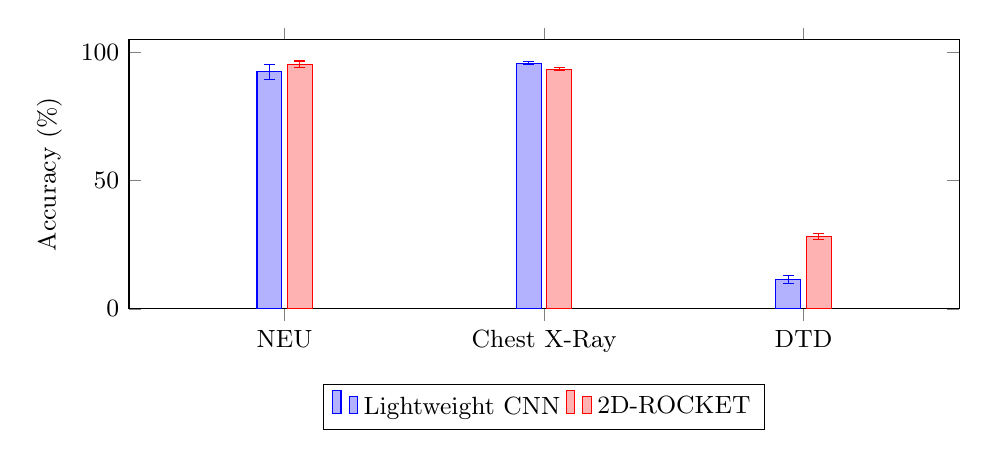
\begin{tikzpicture}
\begin{axis}[
    ybar,
    bar width=9pt,
    width=\linewidth,
    height=5cm,
    symbolic x coords={NEU, Chest X-Ray, DTD},
    xtick=data,
    ymin=0, ymax=105,
    ylabel={Accuracy (\%)},
    ylabel style={font=\small},
    tick label style={font=\small},
    legend style={at={(0.5,-0.28)}, anchor=north, legend columns=-1, font=\small},
    error bars/y dir=both,
    error bars/y explicit,
    enlarge x limits=0.3,
]
\addplot+[error bars/.cd, y dir=both, y explicit]
    coordinates {(NEU,92.50) +- (0,2.96) (Chest X-Ray,95.83) +- (0,0.60) (DTD,11.61) +- (0,1.56)};
\addplot+[error bars/.cd, y dir=both, y explicit]
    coordinates {(NEU,95.47) +- (0,1.25) (Chest X-Ray,93.54) +- (0,0.47) (DTD,28.21) +- (0,1.20)};
\legend{Lightweight CNN, 2D-ROCKET}
\end{axis}
\end{tikzpicture}
\caption{Test accuracy (\%, mean $\pm$ std over 10 seeds) of the lightweight CNN baseline and the final 2D-ROCKET configuration on NEU, Chest X-Ray Pneumonia, and DTD. Differences are statistically significant on all three datasets (paired $t$-test, $n=10$; Table~\ref{tbl:realworld}).}\label{fig:realworld-acc}
\end{figure}

\begin{figure}
\centering
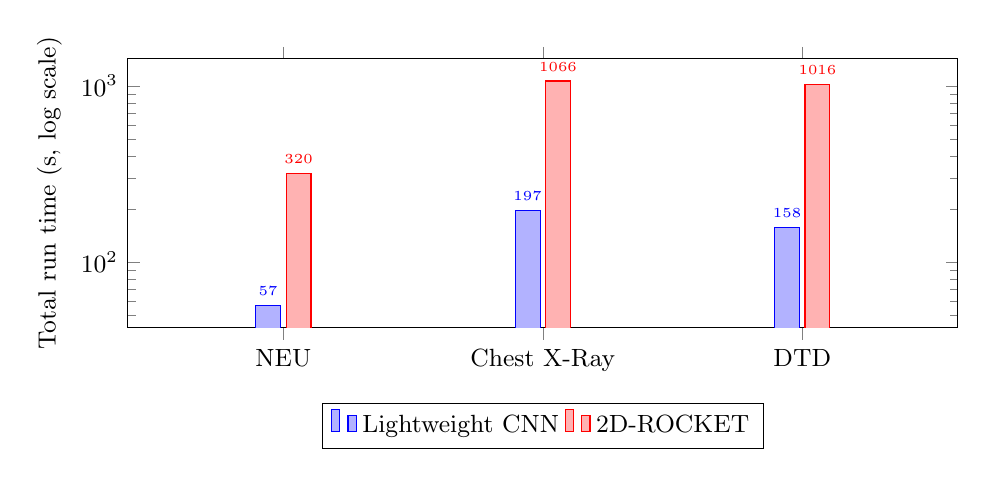
\begin{tikzpicture}
\begin{axis}[
    ybar,
    bar width=9pt,
    width=\linewidth,
    height=5cm,
    symbolic x coords={NEU, Chest X-Ray, DTD},
    xtick=data,
    ymode=log,
    ylabel={Total run time (s, log scale)},
    ylabel style={font=\small},
    tick label style={font=\small},
    legend style={at={(0.5,-0.28)}, anchor=north, legend columns=-1, font=\small},
    point meta=explicit symbolic,
    nodes near coords={\pgfplotspointmeta},
    nodes near coords style={font=\tiny},
    enlarge x limits=0.3,
]
\addplot coordinates {(NEU,57.1)[57] (Chest X-Ray,197.1)[197] (DTD,158.0)[158]};
\addplot coordinates {(NEU,319.7)[320] (Chest X-Ray,1065.5)[1066] (DTD,1015.5)[1016]};
\legend{Lightweight CNN, 2D-ROCKET}
\end{axis}
\end{tikzpicture}
\caption{Total pipeline run time in seconds (log scale; data loading, training/feature extraction, and evaluation, uncached).}\label{fig:realworld-time}
\end{figure}

\begin{figure}
\centering
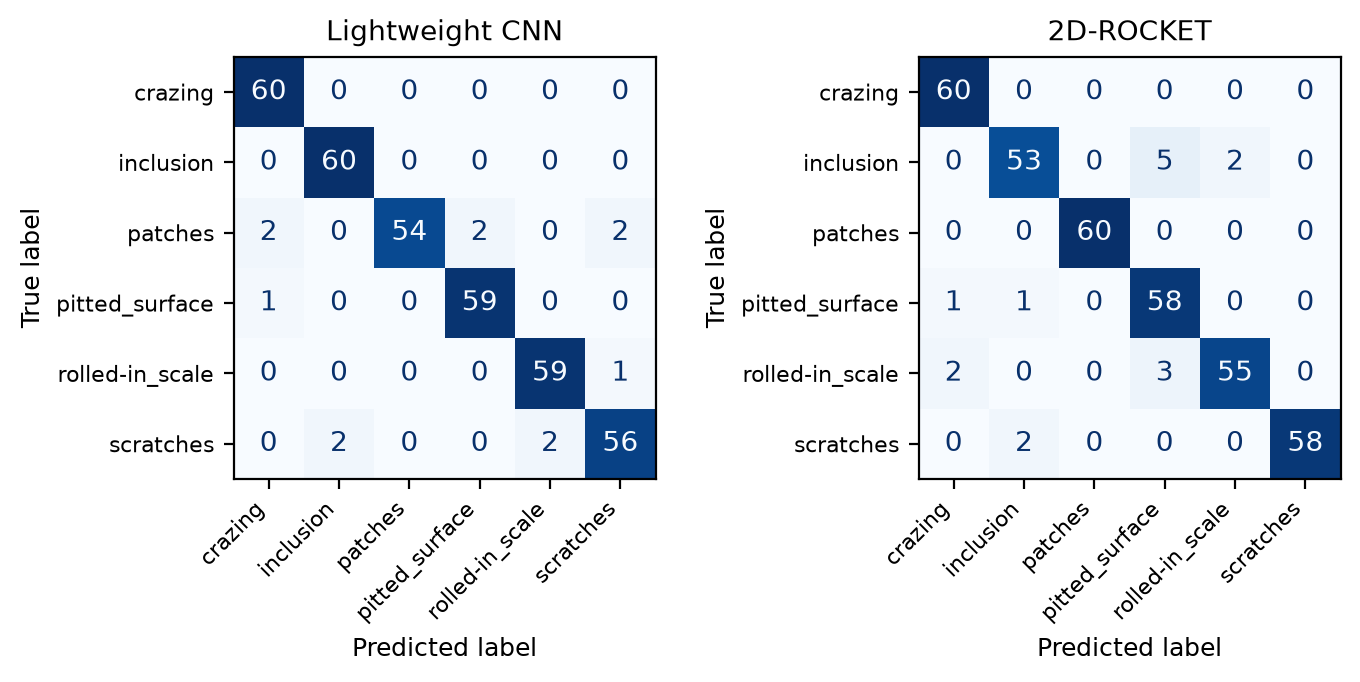
\includegraphics[width=\linewidth]{figures/cm_neu.png}
\caption{NEU confusion matrices for the representative seed-42 run (60 test images per class); see Table~\ref{tbl:realworld} for the full 10-seed accuracy distribution.}\label{fig:cm-neu}
\end{figure}

\begin{figure}
\centering
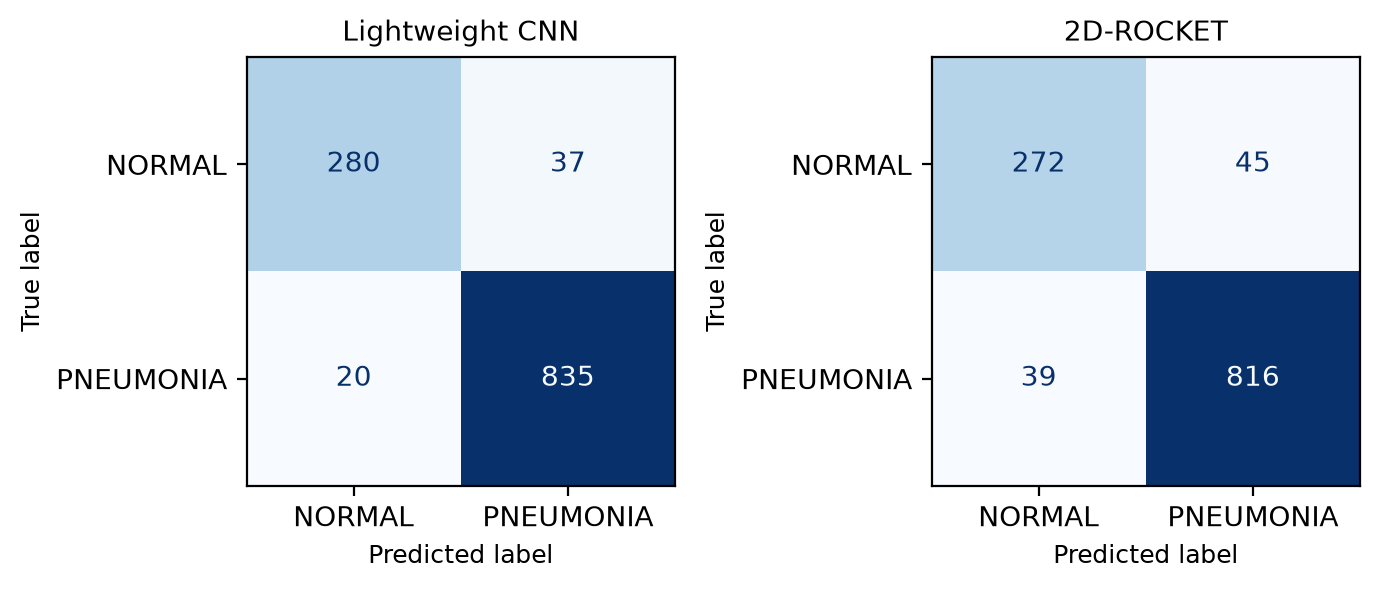
\includegraphics[width=\linewidth]{figures/cm_xray.png}
\caption{Chest X-Ray Pneumonia confusion matrices for the representative seed-42 run (317 NORMAL / 855 PNEUMONIA test images); see Table~\ref{tbl:realworld} for the full 10-seed accuracy distribution.}\label{fig:cm-xray}
\end{figure}

\begin{figure}
\centering
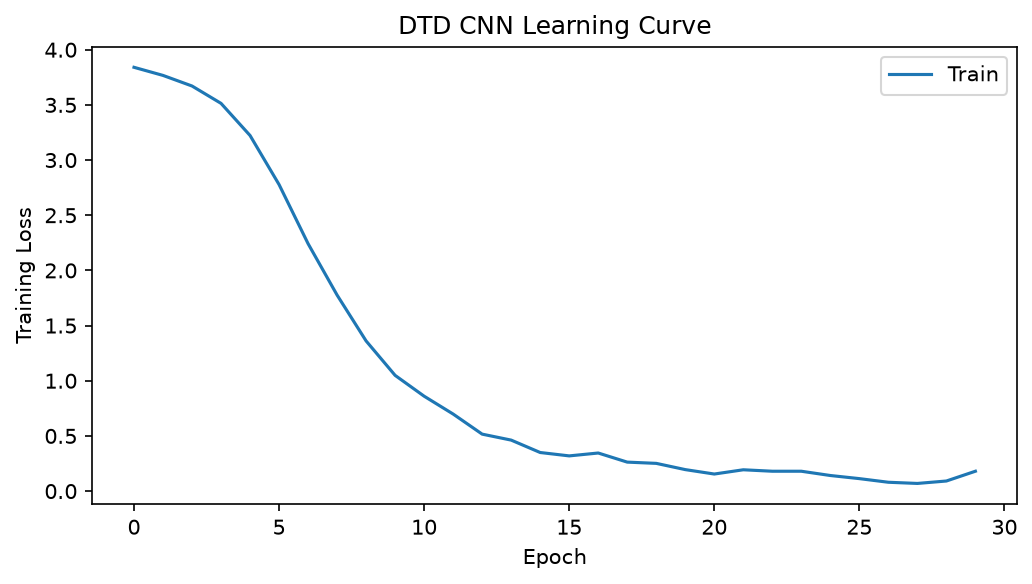
\includegraphics[width=\linewidth]{figures/dtd_cnn_learning_curve.png}
\caption{DTD lightweight-CNN training loss over the full 30-epoch schedule, seed 42. Loss falls below 0.2 with no plateau, consistent with memorizing the $\sim$96 training images available per class (no augmentation is used). This particular seed's 30-epoch test accuracy (8.51\%) turned out to be the lowest of the ten seeds evaluated (mean 11.61\%\std{1.56}, Table~\ref{tbl:realworld}) -- so while the memorization pattern shown here is real, it should not be read as proof that the longer schedule reduced \emph{average} CNN accuracy on DTD; only the single-seed comparison against the original 10-epoch run happened to move in that direction.}\label{fig:dtd-overfit}
\end{figure}

Results are summarized in Table~\ref{tbl:realworld} and Fig.~\ref{fig:realworld-acc}--\ref{fig:dtd-overfit}, and, unlike the rest of this paper, are backed by a paired significance test over ten seeds rather than a single run (Sec.~\ref{sec:realworld}): 2D-ROCKET wins decisively and significantly on two of the three datasets, and loses narrowly but significantly on the third.

On NEU, 2D-ROCKET reaches 95.5\%\std{1.2} against the CNN's 92.5\%\std{3.0} ($p=0.038$), reproducing the pattern already seen on KTH-TIPS, though with a smaller margin and considerably more overlap between the two distributions than a single-seed comparison would suggest -- the CNN's range across seeds (85.8--96.7\%) actually spans 2D-ROCKET's entire range (92.2--96.7\%). Why the CNN is roughly $2.5\times$ more seed-sensitive on NEU than on Chest X-Ray (std 3.0 vs.\ 0.6 points) is not something this experiment diagnoses -- per-seed confusion matrices were not retained during the sweep, so it is not possible after the fact to check whether particular seeds fail on particular classes (NEU's small, six-way, 1{,}440-image training set is a plausible contributor, but this is a conjecture, not a finding, and is flagged as such). Fig.~\ref{fig:cm-neu} shows the seed-42 illustration of this: both models make few, evenly spread errors (at most 2 per off-diagonal cell for the CNN, at most 5 for 2D-ROCKET). Chest X-Ray Pneumonia is the one dataset where the CNN wins, 95.8\%\std{0.6} against 93.5\%\std{0.5} ($p=4.6\times10^{-7}$) -- a smaller absolute gap than NEU's but the most statistically confident result of the three, owing to both methods' low seed-to-seed variance here. The dataset's class imbalance (855 PNEUMONIA vs.\ 317 NORMAL test images, roughly 2.7:1) inflates raw accuracy for whichever method is better at the majority class; macro F1, which weights both classes equally, is reported alongside accuracy in Table~\ref{tbl:realworld} for exactly this reason and shows the same ordering (0.947 vs.\ 0.919), so the conclusion is not an artifact of the imbalance, but accuracy alone should not be read as the primary evidence here. Fig.~\ref{fig:cm-xray} shows the seed-42 gap concentrated in missed pneumonia cases, the clinically costlier error type: the CNN misses 23 of 855 cases (2.7\%) against 2D-ROCKET's 39 (4.6\%).

DTD is the clearest result of the three: 2D-ROCKET reaches 28.2\%\std{1.2} against the CNN's 11.6\%\std{1.6} ($p=3.0\times10^{-10}$), a 16.6-point gap that swamps the seed-to-seed noise on both sides. The training-loss curve in Fig.~\ref{fig:dtd-overfit} (seed 42) shows the 30-epoch CNN memorizing its $\sim$96 training images per class with no augmentation -- a real and, on priors, unsurprising failure mode for a from-scratch CNN at this scale. But a caution is warranted here: that same seed's resulting test accuracy (8.51\%) turned out to be the \emph{lowest} of the ten seeds run, not a typical one, so the specific claim that lengthening the schedule from 10 to 30 epochs \emph{reduced} average CNN accuracy is not well supported by the seed range collected (mean 11.6\%, close to the original single 10-epoch run's 11.52\%); only the memorization pattern itself, not its magnitude of harm, should be taken from that figure. What the ten-seed result does support is the comparison that matters for this paper's argument: on DTD, 2D-ROCKET's ceiling (26.6--30.0\% across seeds) is far above the CNN's (8.5--13.8\%) regardless of which specific epoch budget or seed is chosen, consistent with 2D-ROCKET's fixed-feature, linear-Ridge design being structurally harder to overfit than a from-scratch CNN in a genuinely low-data, per-class regime. One confound is not resolved by this design, however: DTD differs from NEU in class count (47 vs.\ 6) as well as in samples per class, and a from-scratch, two-layer CNN's optimization difficulty plausibly grows with class count on its own, independent of how much data each class has. This experiment cannot separate "97\% fewer classes" from "2.5$\times$ more images per class" as the reason NEU's CNN behaves so much better than DTD's; disentangling the two would need a dataset (or a subsampled version of one) that varies class count and per-class sample size independently, which is left for future work.

2D-ROCKET's total (uncached) run time remains substantially higher than the CNN's on every dataset -- roughly 5--6$\times$ in the single uncontended runs reported in Table~\ref{tbl:realworld} -- since, unlike the cached-feature timings in Table~\ref{tbl:main}, feature-extraction cost is included here. Beyond the ten-seed accuracy distributions themselves, these results still reflect a single, CIFAR-10-tuned configuration with no dataset-specific retuning beyond the uniform epoch-count correction described above, and should be read as a real-world-oriented validation with a genuine (if modest) sample size, not an exhaustive benchmark.

\subsection{Closing the Chest X-Ray gap: restoring positional resolution}\label{sec:lspv}

The Chest X-Ray result invites a specific, testable explanation: PPV, Max, and MPV are pooled over the \emph{entire} activation map per kernel, and MIPV reduces spatial location to a single centroid, so a small, localized pneumonia infiltrate competes for influence against the same rib cage and mediastinal structure present, with similar overall contrast, in every image -- a plausible reason a globally pooled feature bank would struggle with a spatially localized pathology even though it excels on globally textured surfaces. MultiROCKET's fourth statistic, the Local Share of Positive Values (LSPV, Sec.~\ref{sec:related}), was named as a candidate feature in this paper's related-work discussion but, until this point, never implemented: it was added here as an adaptive average-pooling of each kernel's binary activation mask into a $3\times3$ grid of regional PPV values, giving each kernel coarse positional resolution instead of one global number, at the cost of growing the feature dimension from 25{,}000 to 70{,}000.

Re-running 2D-ROCKET with PPV+Max+MPV+MIPV$_y$+MIPV$_x$+LSPV on Chest X-Ray, ten seeds, all other settings unchanged, gives 95.6\%\std{0.4} (macro F1 0.944\std{0.006}), against the CNN's 95.8\%\std{0.6} and the original feature set's 93.5\%\std{0.5} (Table~\ref{tbl:lspv}). The gap to the CNN is no longer statistically significant ($p=0.22$, paired $t$-test, $n=10$), while the improvement over the original feature set is highly significant ($p=2.5\times10^{-7}$). Mean run time (1{,}937\,s) is essentially unchanged from the original feature set's 1{,}993\,s under the same contended, multi-seed execution, since feature extraction -- convolution over the kernel bank -- dominates total cost far more than the Ridge fit or the cheap regional-pooling step LSPV adds. This is a direct, successful test of the mechanistic account above: 2D-ROCKET's weakness on Chest X-Ray was not an inherent property of random-kernel feature extraction, but a specific, identifiable, and cheaply fixable consequence of discarding positional information during pooling.

\begin{table}
\caption{Chest X-Ray Pneumonia: adding the LSPV feature (mean\,$\pm$\,std over 10 seeds; capacity control over 5 seeds, 42--46). $p$-values are paired $t$-tests against 2D-ROCKET+LSPV, matched by seed ($n=10$ for the first two rows, $n=5$ for the capacity control).}\label{tbl:lspv}
\begin{tabular*}{\tblwidth}{@{}lrrl@{}}
\toprule
Method & Accuracy & Macro F1 & $p$ vs.\ +LSPV \\
\midrule
Lightweight CNN     & 0.958\std{0.006} & 0.947\std{0.008} & $0.22$ \\
2D-ROCKET            & 0.935\std{0.005} & 0.919\std{0.006} & $2.5\times10^{-7}$ \\
2D-ROCKET + LSPV & \textbf{0.956}\std{0.004} & \textbf{0.944}\std{0.006} & -- \\
\midrule
2D-ROCKET, 8k kernels, no LSPV & 0.938\std{0.005} & 0.922\std{0.006} & $2.4\times10^{-3}$ \\
\bottomrule
\end{tabular*}
\end{table}

The obvious confound in the comparison above is capacity: LSPV does not just add positional resolution, it also grows the feature dimension from 25,000 to 70,000, and a linear classifier with more features can fit more of anything, position-related or not. This was tested directly with a capacity-matched control: 2D-ROCKET with no LSPV but 8,000 kernels instead of 5,000 (40,000 features -- a partial match to LSPV's 70,000; an exact match at 14,000 kernels was abandoned after a single job's memory footprint approached the evaluation machine's limit), five seeds (42--46, reduced from ten for the same practical reason). This capacity-only control reaches 93.8\%\std{0.5} (Table~\ref{tbl:lspv}) -- significantly \emph{above} the original 5,000-kernel baseline on the same five seeds ($+0.55$ points, $p=2.3\times10^{-4}$, paired), confirming that added capacity does help somewhat on its own, but significantly \emph{below} LSPV on the same five seeds ($-1.50$ points, $p=2.4\times10^{-3}$). Capacity alone therefore accounts for roughly a quarter of LSPV's improvement over the baseline (0.55 of 2.05 points measured on the full ten-seed comparison); the remaining three-quarters is not explained by feature count and is consistent with the positional-resolution mechanism this section set out to test. This is a more precise and more modest claim than "LSPV closes the gap," and a more defensible one.

This result is deliberately narrow in scope beyond the capacity confound just addressed. First, LSPV was added and tested only for Chest X-Ray, the one dataset this paper's own mechanistic argument singled out, and not swept back across NEU, DTD, MNIST, or CIFAR-10, so it is not yet known whether it helps, hurts, or is neutral elsewhere (the risk being that finer positional resolution could reduce the translation-invariance that plausibly helps 2D-ROCKET on texture-dominated data, where the same statistical pattern can appear anywhere in the frame). Second, the $3\times3$ regional grid was fixed a priori rather than tuned or ablated against alternatives (e.g.\ $2\times2$ or $4\times4$); the result shows that \emph{some} positional resolution closes the gap, not that this particular resolution is optimal. It should be read as a targeted confirmation of a specific hypothesis, not as a replacement for the paper's default configuration.

\subsection{SAR radio-frequency interference detection: a genuine time-series test}\label{sec:sar}

Everything so far has applied ROCKET to images -- 2D-ROCKET throughout, and the flattened-1D-sequence baseline in Sec.~\ref{sec:methods}, which is still fundamentally an image reshaped into a sequence. ROCKET was originally designed for genuine time series \citep{dempster2020rocket}, and raw Synthetic Aperture Radar (SAR) data is a natural fit: before image formation, a SAR instrument records a sequence of raw radar echoes, one real time series per transmitted pulse. Radio-frequency interference (RFI) from terrestrial or other satellite emitters is a practical, unsolved data-quality problem for missions like Copernicus Sentinel-1, and detecting it in these raw echoes -- before it propagates into the focused image -- is a genuinely small-data problem in practice, since labeled contamination events are comparatively rare relative to the volume of clean acquisitions. Given the sample-efficiency account developed for DTD (Sec.~\ref{sec:discussion}), this section tests whether that advantage extends to a real, non-image, low-data time-series problem, using the RFInject-v1-L0 dataset \citep{delprete2025rfinject}, an ESA $\Phi$-lab collection of Sentinel-1 Level-0 raw bursts with simulated RFI additively injected and stored separately from the clean baseline echo, enabling exact clean/contaminated pairs on the same underlying signal.

One Sentinel-1 IW burst (102 azimuth lines, 19{,}654 complex range samples per line) was used, with 11 of its 15 provided interference realizations containing non-zero injected energy (the remaining four are empty placeholders). A first version of this experiment built one contaminated example per line by pairing it with a randomly chosen non-empty realization; this produced classifiers with accuracy far \emph{below} chance (12--20\%) across all three methods tested below, which turned out not to be a modeling failure but a labeling one: interference in this dataset is sparse not only across range samples within a line (as expected) but across azimuth lines too, and 93 of 102 lines under that random pairing received a realization with literally zero injected energy at that specific line, despite the realization being non-empty elsewhere in the burst -- mislabeling most "contaminated" examples as positive when they were pixel-identical to clean. All three independently implemented classifiers were, in fact, learning correctly and scoring nearly 90\% against the \emph{true} labels once this was checked directly; the below-chance numbers were an artifact of comparing correct predictions to systematically wrong labels, not evidence the task was unlearnable. The dataset was rebuilt using only genuine (line, realization) pairs with verified non-zero injected energy -- 114 such pairs -- against the burst's 102 original clean lines, giving 216 examples total. This episode is reported in full because it is a direct, concrete illustration of exactly the failure mode -- an experiment silently returning a coherent-looking but wrong number -- that this paper's broader push toward multi-seed, cross-checked evaluation (Sec.~\ref{sec:realworld}) exists to catch, and here it surfaced through cross-model, not cross-seed, agreement: three unrelated methods agreeing on being wrong was the tell.

Each of the 216 lines (magnitude of the complex signal) was block-max-pooled by a factor of 4 (preserving sparse, localized interference peaks better than block-averaging would) to 4{,}913 samples and per-series $z$-normalized, following standard ROCKET preprocessing practice. This is deliberately not a large dataset: 216 examples, no augmentation, a single burst -- precisely the low-data regime in which Sec.~\ref{sec:discussion} argues 2D-ROCKET's fixed-feature, linear-Ridge design should have a structural advantage over a from-scratch CNN. Three methods, freshly implemented for this section, are compared over 10 seeds (an 80/20 stratified split reseeded jointly with model initialization, as in Sec.~\ref{sec:realworld}): a genuine 1D-ROCKET (kernel lengths $\{7,9,11\}$, dilations $\{1,2,4\}$, a random per-kernel choice of \emph{same} or \emph{valid} padding, PPV+Max pooling, $N=5{,}000$ kernels, RidgeClassifier -- matching Dempster et al.'s original design rather than this paper's 2D adaptation), a shallow 1D CNN (two convolutional layers, mirroring the 2D CNN baseline's design, 30 epochs), and a linear SVM (flattened, standardized signal, $C=0.1$, matching the SVM baseline methodology used throughout this paper).

\begin{table}
\caption{SAR RFI detection (clean vs.\ contaminated echo lines): mean\,$\pm$\,std over 10 seeds, $n=216$ examples total. $p$-values are paired $t$-tests ($n=10$) against 1D-ROCKET.}\label{tbl:sar}
\begin{tabular*}{\tblwidth}{@{}lrrl@{}}
\toprule
Method & Accuracy & Macro F1 & $p$ vs.\ ROCKET \\
\midrule
Linear SVM  & 0.768\std{0.059} & 0.767\std{0.061} & $0.026$ \\
1D-ROCKET    & 0.802\std{0.038} & 0.802\std{0.038} & -- \\
1D CNN       & \textbf{0.836}\std{0.040} & \textbf{0.836}\std{0.040} & $1.7\times10^{-3}$ \\
\bottomrule
\end{tabular*}
\end{table}

\begin{figure}
\centering
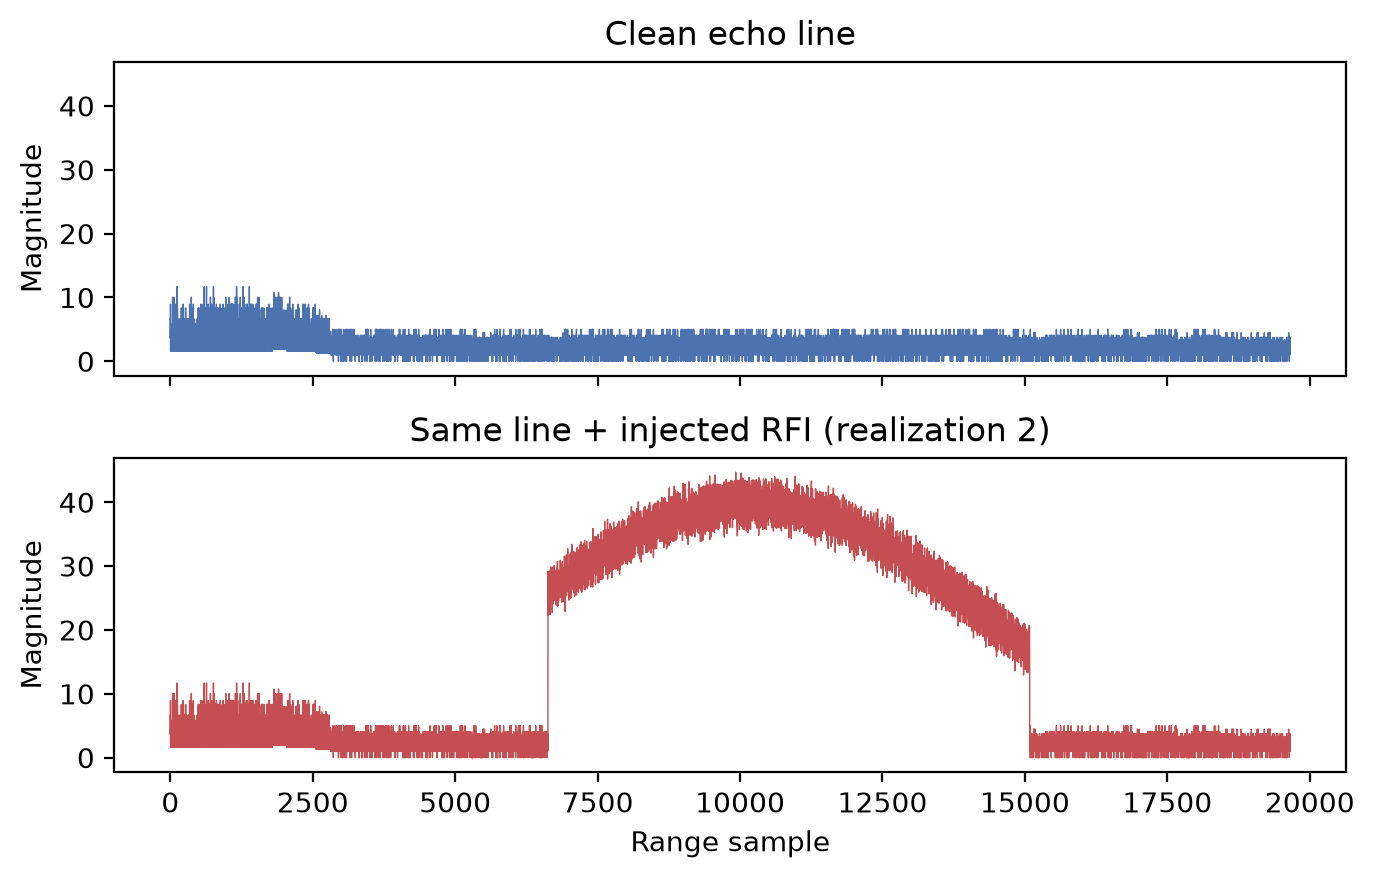
\includegraphics[width=\linewidth]{figures/sar_example_signal.png}
\caption{Magnitude of one raw Sentinel-1 echo line before and after additive RFI injection. The injected interferer raises the local energy envelope by roughly $4$--$5\times$ over a contiguous span of the line -- a spatially localized anomaly, not a texture.}\label{fig:sar-signal}
\end{figure}

\begin{figure}
\centering
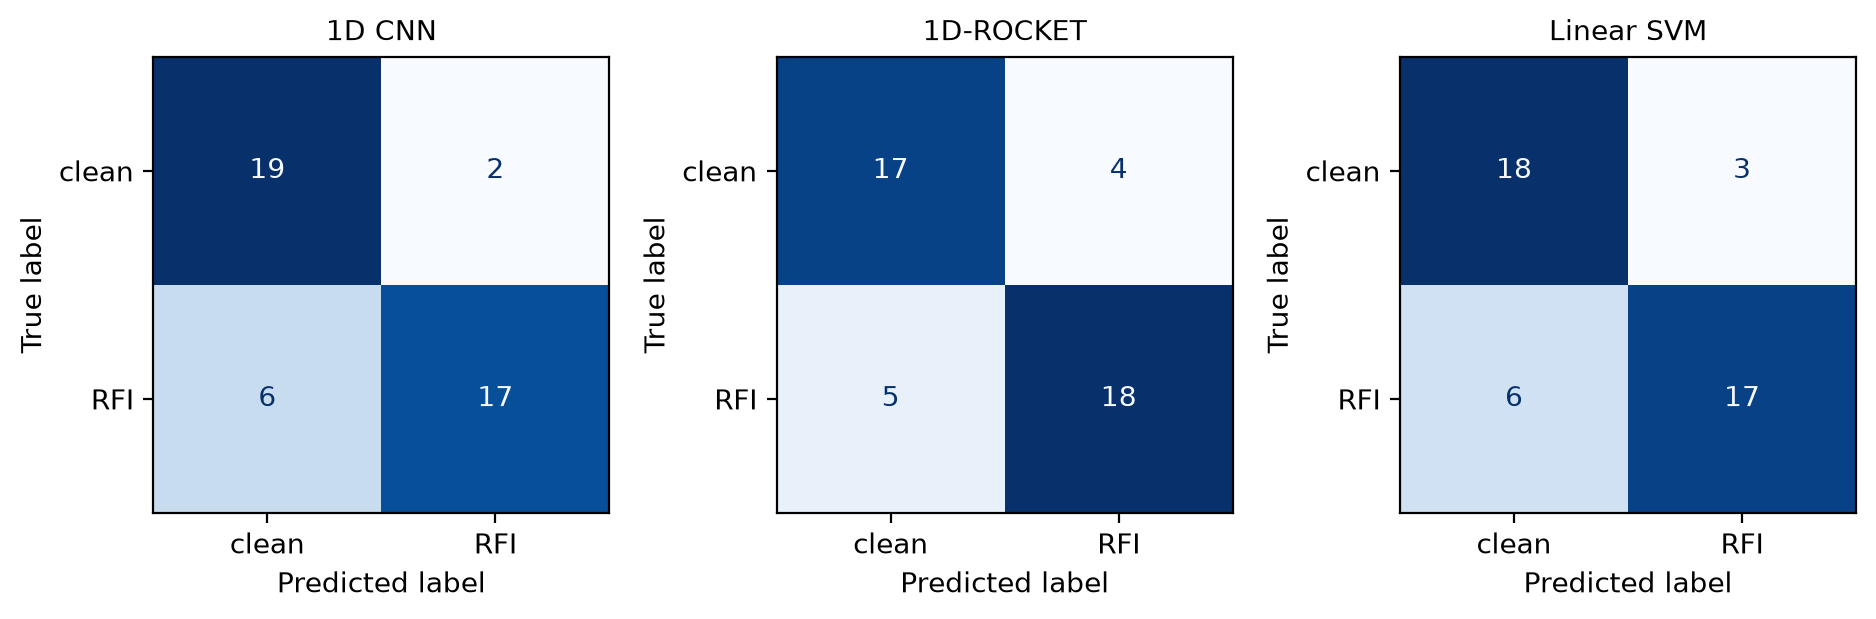
\includegraphics[width=\linewidth]{figures/sar_confusion_matrices.png}
\caption{SAR RFI detection confusion matrices for the representative seed-42 split (22 clean / 22 RFI test examples).}\label{fig:sar-cm}
\end{figure}

Results are summarized in Table~\ref{tbl:sar}. 1D-ROCKET reaches 80.2\%\std{3.8}, significantly ahead of the linear SVM (76.8\%\std{5.9}, $p=0.026$) -- a result consistent with the rest of this paper: a large bank of random kernels with simple pooling statistics again outperforms a linear model over raw (here, flattened) features. It does not, however, beat the CNN: the 1D CNN reaches 83.6\%\std{4.0}, significantly ahead of 1D-ROCKET ($p=1.7\times10^{-3}$). This does not confirm the sample-efficiency hypothesis that motivated this section, but it is not inconsistent with the account in Sec.~\ref{sec:discussion} either, once the task is examined rather than just its size: Fig.~\ref{fig:sar-signal} shows that RFI in this data manifests as a spatially localized anomaly -- an elevated-energy span over part of the line -- structurally the same kind of problem as Chest X-Ray Pneumonia's localized opacity (Sec.~\ref{sec:realworld}), not a texture repeated statistically across the whole signal. A CNN's learned, position-adaptive filters are, on this account, well suited to exactly this pattern regardless of the number of training examples, whereas 1D-ROCKET's PPV and Max features, though not blind to a strong localized peak (Max in particular should respond to one), still summarize each kernel's response as a single global number per series. This reframes the DTD-derived hypothesis: low-data alone does not guarantee a 2D/1D-ROCKET advantage -- it is low data \emph{combined with} a texture-like rather than localized-anomaly target that does, and this section's small sample size (216 examples, comparable in order of magnitude to DTD's training set) makes that distinction cleanly visible where a texture-dominated small dataset would not have.

This result should be read as an initial proof of concept, not a definitive verdict on ROCKET for SAR RFI detection, for several concrete reasons. It rests on a single burst and a single interference-injection source; no claim is made about generalization across bursts, sensors, or real (non-simulated) interference. The $4\times$ block-max downsampling factor and the choice of block-max over alternative pooling (e.g.\ block-mean, or no downsampling at all) were not ablated. And, following the pattern in Sec.~\ref{sec:lspv}, a natural next step -- not attempted here -- would be to add LSPV-style regional pooling to 1D-ROCKET, restoring some positional resolution and testing whether that narrows or closes the gap to the CNN here as it did for Chest X-Ray.

\section{Discussion}\label{sec:discussion}

The ablations indicate that most of 2D-ROCKET's discriminative power comes from a small, targeted set of local statistics: PPV and Max alone already capture the bulk of the signal, and additional statistics yield incremental gains at a clear feature-dimension and runtime cost. Preserving spatial structure via genuine 2D convolutions, rather than flattening images into 1D sequences, is the single largest architectural lever, particularly on CIFAR-10 where spatial and color structure is more informative than on MNIST's simple binary-like strokes. Kernel \emph{configuration} (mixed sizes with moderate dilation) matters more than raw kernel \emph{count}: multi-scale coverage consistently beats single-scale or heavily dilated banks, and accuracy plateaus once the kernel budget exceeds roughly 5,000, after which feature dimensionality and training time keep growing with little additional benefit. Padding behaves as a cheap, implementation-level regularizer: restrictive (valid) padding discards many boundary/large-receptive-field features that turn out to be largely redundant for these datasets, reducing cost without hurting accuracy. Preprocessing choices, by contrast, are dataset-dependent -- per-image normalization is neutral on grayscale digits but actively harmful on natural color images, since it removes inter-image color cues that carry class information.

Relative to the baselines, 2D-ROCKET slightly outperforms the lightweight CNN on both datasets (by 0.35 points on MNIST, 3.81 points on CIFAR-10) while requiring no gradient-based training of its feature extractor. This result has to be read in light of what the CNN baseline actually is: two convolutional layers, no batch normalization, no augmentation, chosen deliberately to keep its complexity comparable to the other lightweight baselines (Sec.~\ref{sec:methods}). Such a shallow network itself composes features across only two layers and therefore exercises little of the deep, multi-scale hierarchical composition -- stacking many layers so that later ones respond to combinations of earlier, smaller-scale features -- that characterizes deeper CNN architectures (e.g., ResNets), which were explicitly excluded from this study's scope. Beating this particular baseline is consequently not evidence that 2D-ROCKET's flat, single-stage design can match deep, multi-scale CNNs in general: 2D-ROCKET has no mechanism at all for combining kernel responses across stages into higher-order, compositional features, whereas even a moderately deep CNN does. On object-recognition tasks where classes are distinguished by exactly this kind of multi-scale, compositional structure, a genuinely deep CNN would be expected to open a gap that no amount of additional random 2D-ROCKET kernels can close, since kernel count and diversity scale the width of a single stage, not its depth. 2D-ROCKET does, however, decisively outperform the linear SVM in both accuracy and training time on both datasets (the SVM takes roughly two hours per dataset, dominated by kernel-free but high-dimensional optimization, versus under two minutes for 2D-ROCKET's classifier fit). This positions 2D-ROCKET as an attractive middle ground for the right kind of data: more expressive than classical handcrafted-feature pipelines, cheaper to train and more transparent than a CNN, but only where classification does not hinge on hierarchical, multi-scale composition.

The strongest practical case for the approach is suggested by the KTH-TIPS result: on a texture-dominated dataset, where local, repetitive statistics rather than multi-scale object composition drive classification, 2D-ROCKET's advantage over both baselines is far larger than on MNIST/CIFAR-10 -- including over the CNN, which gains comparatively little from its hierarchical structure when there is no object hierarchy to compose. This is consistent with the intuition that random local filters combined with simple statistics are naturally well matched to repetitive, texture-like structure -- the kind found in industrial surface inspection, material classification, or other structured imaging domains -- even without any domain-specific tuning, and it is this regime, not general object recognition, that the method is proposed for.

The extended, ten-seed real-world evaluation on NEU, Chest X-Ray Pneumonia, and DTD (Sec.~\ref{sec:realworld}) refines this paper's texture-domain narrative rather than overturning it: 2D-ROCKET wins significantly on NEU and DTD and loses significantly, by a smaller margin, on Chest X-Ray Pneumonia. Two largely separate factors appear to drive this, and DTD is where they compound: (i) \emph{texture-likeness} of the classification target -- NEU (surface-defect texture) and DTD (texture attributes by construction) favor 2D-ROCKET's flat bank of local statistics, while Chest X-Ray Pneumonia, diagnosed from spatially localized opacity patterns rather than repetitive texture, favors the CNN's learned, spatially adaptive filters; and (ii) \emph{sample scarcity without augmentation} -- DTD offers only about 96 training images per class, a regime in which the from-scratch CNN memorizes rather than generalizes (Fig.~\ref{fig:dtd-overfit}), while 2D-ROCKET's only trained component, a linear Ridge fit over 25,000 fixed random features, is structurally harder to overfit. NEU, with roughly 240 training images per class, is not a low-data regime in the same sense -- the CNN there reaches a respectable 92.5\% mean accuracy, nothing like DTD's collapse -- so 2D-ROCKET's win on NEU is better attributed to factor (i) alone, while DTD's much larger margin (16.6 points, versus NEU's 3.0) reflects both factors acting together. This two-factor account is more defensible than either a pure texture-domain or a pure sample-efficiency explanation alone, and it is exactly the kind of distinction a single-seed, single-dataset comparison cannot make. It also generates a falsifiable prediction rather than just a post-hoc story: if factor (i)'s mechanism is really the loss of positional information in global pooling, then restoring positional resolution should narrow the Chest X-Ray gap specifically. Sec.~\ref{sec:lspv} tests this directly by adding the previously unimplemented LSPV feature and confirms it, with a capacity-matched control ruling out the obvious alternative explanation: the CNN's advantage drops from significant ($p=4.6\times10^{-7}$) to statistically indistinguishable ($p=0.22$) with no meaningful runtime cost, and a same-feature-count control without LSPV recovers only about a quarter of that gain, leaving the rest attributable to positional resolution specifically rather than to added feature capacity in general -- stronger, more precisely apportioned support for the positional-pooling explanation than the correlational evidence in this paragraph alone.

Sec.~\ref{sec:sar} provides a third, independent test of this account, in a genuinely different data modality (raw 1D SAR time series rather than images) chosen specifically to probe factor (ii) in isolation: with only 216 labeled examples, SAR RFI detection is a smaller training set than either NEU or DTD, so a naive reading of factor (ii) alone would predict 1D-ROCKET should win easily. It does not -- a CNN wins there too ($p=1.7\times10^{-3}$ over 1D-ROCKET) -- and the reason is informative rather than contradictory: the target in that task is a spatially localized energy anomaly (Fig.~\ref{fig:sar-signal}), the same structural category as Chest X-Ray's localized opacities, not a texture. This is exactly what the two-factor account predicts once both factors are considered jointly rather than substituting one for the other: low data alone, without factor (i)'s texture-likeness condition also holding, is not sufficient for a ROCKET-family advantage. Three of the four combinations of the two factors have now been observed directly -- texture-plus-adequate-data (NEU), texture-plus-scarce-data (DTD), and non-texture-plus-scarce-data (SAR RFI) -- with only non-texture-plus-adequate-data (Chest X-Ray Pneumonia) representing the fourth cell, completing a small but genuine $2\times2$ probe of the hypothesis rather than a single-axis one.

Limitations include single-seed evaluation for the MNIST/CIFAR-10/KTH-TIPS study and its ablation chain (small effect sizes, especially on near-saturated MNIST, should be treated cautiously without multi-seed replication -- unlike Sec.~\ref{sec:realworld}, which was re-run over ten seeds specifically because a single seed there was twice found to be misleading), a fixed Ridge classifier with a regularization strength ($\alpha=1200$) tuned once on MNIST/CIFAR-10-scale data (tens of thousands of training images) and never re-tuned for the much smaller real-world training sets in Sec.~\ref{sec:realworld} or the larger, 70,000-dimensional LSPV feature space in Sec.~\ref{sec:lspv} (isolating feature quality but excluding gains from alternative or better-tuned classifiers), deliberately simple baselines (a more heavily tuned SVM or CNN could narrow the observed gaps), and growing memory/numerical-conditioning pressure as feature dimensionality reaches the tens of thousands. The paired $t$-tests in Sec.~\ref{sec:realworld} also warrant a methodological caveat of their own: with $n=10$ seeds, normality of the paired accuracy differences is assumed rather than verified, and because the train/test split is reseeded jointly with model initialization, seed-to-seed variance reflects both model-fitting variability and test-set-composition variability without a way to separate the two from this design alone.

\section{Conclusion}\label{sec:conclusion}

This work adapted ROCKET's random-kernel, statistics-based paradigm from one-dimensional time series to two-dimensional image classification. Preserving spatial structure through genuine 2D convolutions, combined with a compact set of aggregation statistics (PPV, Max, MPV, MIPV) and a multi-scale, moderately dilated kernel bank, is the key design choice that makes 2D-ROCKET effective within a single flat feature-extraction stage. The resulting pipeline reaches 99.41\% accuracy on MNIST and 73.43\% on CIFAR-10 without any learned convolutional weights, and slightly outperforms a deliberately shallow, two-layer CNN baseline on both datasets, in addition to clearly outperforming a linear SVM in accuracy and training time. This should not be over-interpreted: the shallow CNN baseline itself makes limited use of the deep, layered composition that lets genuinely deep networks assemble multi-scale object representations, and such deeper architectures were out of scope for this comparison. Given its flat, single-stage architecture, 2D-ROCKET has no mechanism to close that kind of gap regardless of kernel count, and this paper does \emph{not} propose it as a competitor to deep CNNs on natural-object image classification. A proof-of-concept on the texture-dominated KTH-TIPS dataset (94.7\% vs.\ 43.5\%/52.4\% for SVM/CNN) instead points to the domain where the approach is intended and most effective: repetitive, texture-like image data -- material and surface textures, inspection imagery, and similar structured signals -- where local statistics rather than composed, multi-scale object structure drive classification, and where the architectural advantage of deep networks over a flat random-feature bank is far smaller.

2D-ROCKET is best understood as a lightweight, reproducible, and interpretable baseline for texture-dominated and/or low-data, low-augmentation regimes, not as a replacement for deep networks on general vision tasks that require multi-scale object composition. The systematic, real-world, ten-seed evaluation called for by this scope was carried out in Sec.~\ref{sec:realworld}: the unmodified, CIFAR-10-tuned 2D-ROCKET configuration was applied to industrial surface-defect (NEU), texture-attribute (DTD), and medical (Chest X-Ray Pneumonia) imagery, and won with statistical significance ($p<0.05$) on two of the three datasets, losing narrowly but significantly only on the non-texture, structurally driven Chest X-Ray task. The size of 2D-ROCKET's advantage tracked both texture-likeness and per-class sample scarcity, with DTD's combination of both factors producing by far the largest margin (16.6 points, $p=3\times10^{-10}$) -- a more nuanced and better-supported account of 2D-ROCKET's real-world niche than either factor alone, and one this paper would not have reached without first observing, and then correcting for, how much a single training seed could change the apparent conclusion on more than one of these datasets. The texture-likeness explanation was, moreover, tested rather than merely asserted: adding the previously unimplemented LSPV feature (Sec.~\ref{sec:lspv}) to restore coarse positional resolution closed the significant Chest X-Ray gap to statistical indistinguishability from the CNN ($p=0.22$) at no meaningful runtime cost. A capacity-matched control (more kernels, no LSPV, same feature count) attributes only about a quarter of that gain to added capacity and the rest specifically to positional resolution, so the loss of location information in global pooling -- not some more fundamental limit of random-kernel feature extraction, and not merely a larger feature bank -- is the best-supported explanation for 2D-ROCKET's one loss in this evaluation. Sec.~\ref{sec:sar} extended this test to genuine 1D time series -- raw Sentinel-1 SAR echo lines, using a freshly implemented, Dempster-et-al.-faithful 1D-ROCKET rather than this paper's 2D adaptation -- on a deliberately small (216-example) radio-frequency-interference detection task chosen to test the sample-scarcity factor in isolation from texture-likeness. 1D-ROCKET significantly outperformed a linear SVM there, replicating the pattern seen throughout this paper, but a CNN significantly outperformed 1D-ROCKET in turn: the interference in this data is a spatially localized energy anomaly rather than a texture, and the two-factor account correctly anticipates a CNN advantage in exactly that combination (scarce data, non-texture target) once both factors are read jointly rather than treating sample scarcity as sufficient on its own. Remaining promising directions for future work include multi-seed statistical validation for the MNIST/CIFAR-10/KTH-TIPS ablation chain itself (which, unlike Sec.~\ref{sec:realworld}, still rests on single runs), sweeping LSPV (and its grid resolution) back across the texture-dominated datasets to check whether it helps, hurts, or is neutral where translation invariance rather than localization is likely to matter, domain-aware or structured (rather than purely random) kernel sampling, hybrid pipelines that combine random convolutions with a small trainable component to recover some hierarchical composition, dimensionality reduction to control feature-storage cost at large kernel budgets, and a systematic study that varies training-set size and augmentation directly and independently of texture content to further disentangle the two factors identified in Sec.~\ref{sec:discussion}.

\section*{Data and Code Availability}
Code for the real-world validation study (Sec.~\ref{sec:realworld}), the LSPV feature (Sec.~\ref{sec:lspv}) and its capacity-control experiment, and the SAR RFI detection study (Sec.~\ref{sec:sar}), including the exact scripts used to produce Tables~\ref{tbl:realworld}--\ref{tbl:sar} and Figs.~\ref{fig:realworld-acc}--\ref{fig:sar-cm}, is available in the accompanying repository (see \texttt{docs/REPRODUCING.md} for step-by-step instructions). NEU, Chest X-Ray Pneumonia, and DTD are third-party datasets accessed via their public Kaggle mirrors and are not redistributed; the SAR burst used in Sec.~\ref{sec:sar} is from the third-party, public RFInject-v1-L0 Hugging Face bucket \citep{delprete2025rfinject} and is likewise not redistributed. The MNIST/CIFAR-10/KTH-TIPS ablation study underlying Table~\ref{tbl:main} and Sec.~\ref{sec:results} up to Sec.~\ref{sec:realworld} was conducted separately from this repository and is not reproducible from the code released alongside this paper; it is documented in the corresponding bachelor thesis.

\printcredits

\bibliographystyle{cas-model2-names}
\bibliography{cas-refs}

\end{document}
